\section{Résultats} % (fold)
\label{sec:résultats}

\paragraph{Polymorphisme.} % (fold)
\label{par:polymorphisme}
Nous retrouvons des profils similaires à ceux déjà obtenus auparavent\cite{memHH}, enrichis de nouvelles lignées pour les espèces déjà typées en transposon-display, et d’espèces typées pour la première fois, comme \esp{D. auraria}, \esp{D. triauraria} et \esp{D. suzukii}.
La figure \ref{fig:profils} montre un exemple de chacun de ces profils, sachant qu’il n’y avait aucune variabilité visible au sein de ceux-ci, sauf pour \esp{wMel}, qui présente un fragment de plus % Nombre de pb ?
dans certaines populations.

\begin{figure}[tb]
	\begin{center}
		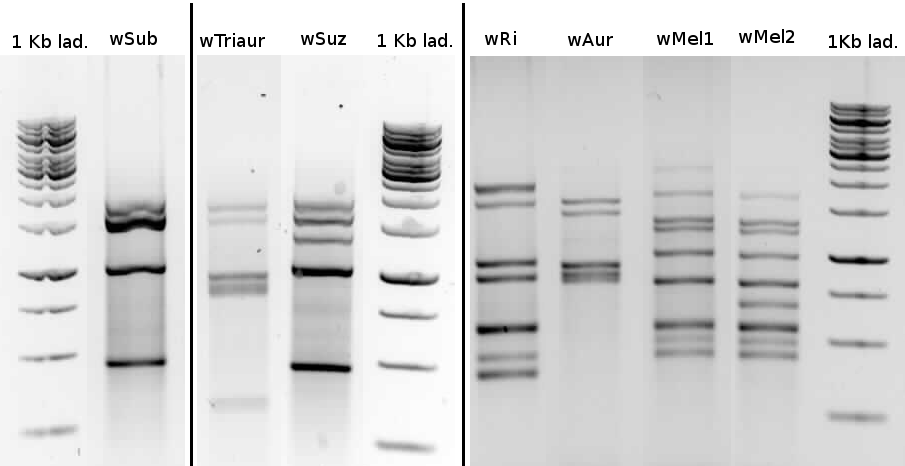
\includegraphics[width=150mm]{images/profils_crop.png}
	\end{center}
	\caption{Reconstruction d'un gel représentant tous les profils carractéristiques des souches de \esp{Wolbachia} en transposon-display avec les amorces Isb/LNP.}
	\label{fig:profils}
\end{figure}

% paragraph polymorphisme (end)

\paragraph{Une amélioration nette du protocole.} % (fold)
\label{par:proto}
Un des éléments notables dans les gels d'éléctrophorèse obtenus est la nette amélioration de l'amplification des fragments de grande taille, notamment pour les profils de type \textit{wMel} (Cf. Figure \ref{fig:wMelcomp}). 
\begin{figure}[tb]
	\begin{center}
		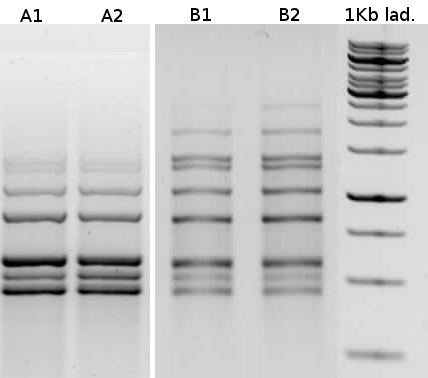
\includegraphics[width=80mm]{images/wMel_comp.png}
	\end{center}
	\caption{Comparaison des deux protocoles sur wMel (\esp{Wolbachia} de \esp{D. melanogaster})~:
	A1 et A2 : Ancien protocole\cite{memHH}~;
	B1 et B2 : Nouveau protocole, avec accuTaq}
	\label{fig:wMelcomp}
\end{figure}
% paragraph proto (end)

% section r_sultats (end)

\section{Conclusion \& Perspectives} % (fold)
\label{sec:ccl}
Afin de tirer des conclusions complètes sur les tranferts horizontaux, il faut encore attendre les résultats de transposon-display sur des lignées de \esp{L. heterotoma} infectées par une seule souche de \esp{Wolbachia}.
Nous ne possédons pas encore ces lignées, mais une seconde partie de ce stage, non développée ici; a consisté à démarrer un traitement antibiotique ménagé sur des \esp{L. heterotoma} tri-infectées (statut d'infection sauvage), afin d'obtenir des lignées présentant un statut d'infection différent pour enfin les typer en transposon-display.

La suite de ce travail consistera à séquencer les fragments obtenus afin de situer précisément les insertions dans le génome, afin d’éventuellement en tirer des conclusions sur les conséquences physiologiques des différentes insertions du transposon. Peut-être trouverons-nous là une piste pour expliquer l’adaptabilité exceptionnelle de \esp{Wolbachia} aux changements d’hôtes ?
% section conclusion_&_perspectives (end)
